% Working manuscript based on the supplied CSPC paper template.
% Replace author/contribution/repository placeholders and review all text before submission.
\documentclass[sigconf,nonacm]{acmart}

\settopmatter{printacmref=false}
\renewcommand\footnotetextcopyrightpermission[1]{}
\pagestyle{plain}

\usepackage{graphicx}
\usepackage{booktabs}
\usepackage{url}

\title{P--S Timing, Source Distance, and Signal Quality in STEAD}

% TODO: replace these author blocks with the registered team members and emails.
\author{Team Member 1}
\affiliation{\institution{UFAZ}\country{Azerbaijan}}
\email{member1@example.com}

\author{Team Member 2}
\affiliation{\institution{UFAZ}\country{Azerbaijan}}
\email{member2@example.com}
% Add or remove author blocks to match the registered team.

\begin{document}

\begin{abstract}
We examine whether STEAD earthquake metadata can support estimates of source-to-station distance and explain variation in signal-to-noise ratio (SNR). The supplied metadata archive contains 1,265,657 traces, including 1,030,231 local-earthquake records. For distance estimation, we compare linear, quadratic, and depth-aware fits of source distance to the P--S arrival-time difference, evaluating them on a 20\% event-level holdout. The depth-aware model achieves a held-out mean absolute error (MAE) of 4.87 km and an $R^2$ of 0.961, compared with 5.82 km and 0.946 for the linear timing-only fit. For local-magnitude (ML) events, an event-level regression estimates an adjusted association of 8.66 dB higher median SNR per magnitude unit (95\% confidence interval: 8.61--8.71; $p<0.001$). The analysis shows that depth improves this simple metadata-based distance model, while magnitude remains associated with SNR after controlling for distance and depth. The archive contains metadata only, so no waveform or FFT analysis is claimed.
\end{abstract}

\maketitle

\section{Introduction}
Seismic stations record earthquake waves at different distances, and the separation between P- and S-wave arrivals provides a useful timing measure related to source distance. In practice, travel times also depend on source depth and the velocity structure along the propagation path. Recent regional earthquake catalog work uses manually picked P and S phases together with velocity models when relocating events, illustrating the importance of those factors in distance-related inference \cite{holmgren}.

Signal quality also varies with event size and propagation conditions. Modeling and observations show that magnitude, source--receiver distance, attenuation, instrument response, and noise can all affect seismic signal-to-noise ratio \cite{kwiatek}. These effects motivate examining magnitude together with distance and depth rather than treating SNR as a function of magnitude alone.

The STanford EArthquake Dataset (STEAD) is a large labeled collection of earthquake and non-earthquake records with phase and source metadata \cite{stead}. This project uses its supplied metadata archive to address two questions: (1) how accurately can the P--S arrival-time difference estimate source-to-station distance, and does source depth improve that estimate; and (2) for ML events, is magnitude associated with SNR after accounting for distance and depth? The analysis uses curve fitting and regression on the available metadata.

\section{Related Work}
Mousavi et al. introduced STEAD as a global dataset of local-earthquake and noise records, with associated source, receiver, phase, and signal-quality metadata \cite{stead}. The dataset enables analysis across many networks, although the metadata archive used here does not include the waveform arrays.

Holmgren et al. compiled a regional ground-motion database and used P- and S-wave picks with alternative velocity models to relocate earthquakes; their work also examines empirical S--P timing in relation to source distance \cite{holmgren}. This supports treating source depth and regional travel-time variation as relevant covariates when fitting a simple timing-based distance model.

Kwiatek and Ben-Zion studied earthquake detectability and source characterization across magnitude, path, sensor, and noise conditions. Their results emphasize that recorded SNR reflects more than source magnitude alone \cite{kwiatek}. Our analysis tests an adjusted magnitude--SNR association in STEAD metadata, but it does not recover the waveform-level physical effects modeled in that work.

\section{Data}
The data source is the STEAD dataset page on Kaggle \cite{kaggle}; the original authors' repository describes the metadata CSV and the separately distributed HDF5 waveform files \cite{stead}. The local archive supplied for this project contains one CSV metadata file and no waveform arrays.

The CSV has 1,265,657 trace rows: 1,030,231 labeled \texttt{earthquake\_local} and 235,426 labeled \texttt{noise}. Noise rows have no earthquake magnitude, source distance, or P/S arrival picks. For RQ1, 1,030,182 earthquake traces remained after requiring finite distance, depth, P/S sample indices, and a non-empty event identifier; they represent 441,686 distinct \texttt{source\_id} values. For RQ2, the ML-scale, complete-case subset contains 724,790 traces aggregated to 259,817 distinct events.

The metadata records P- and S-arrival sample indices. The S--P interval was calculated from their difference using the dataset's 100 Hz sampling rate. Each trace's three component SNR values were summarized by their median. The RQ2 analysis then used the median trace SNR, magnitude, distance, and depth for each event. Magnitude analyses were restricted to \texttt{source\_magnitude\_type = ml} to avoid mixing magnitude scales. The archive and dataset links are also documented in the project README.

\section{Methods}
The CSV was read with pandas. NumPy was used to derive the S--P interval and calculate evaluation metrics; SciPy's \texttt{curve\_fit} was used for the fitted models; and Matplotlib produced the figures. The project pins the requested analysis-library versions in \texttt{requirements.txt}.

The reported run used Python 3.11.16, NumPy 1.26.4, SciPy 1.13.0, pandas 2.2.1, and Matplotlib 3.8.4, as recorded by the pipeline. The Snakemake workflow is pinned at 7.32.4, with PuLP 2.7.0 pinned for compatibility.

For RQ1, distance $d$ was modeled from S--P time $\Delta t$ using three forms:
\begin{align}
 d &= \beta_0 + \beta_1\Delta t, \\
 d &= \beta_0 + \beta_1\Delta t + \beta_2(\Delta t)^2, \\
 d &= \beta_0 + \beta_1\Delta t + \beta_2 h,
\end{align}
where $h$ is source depth. Events, rather than individual traces, were assigned to an 80\% training set and a 20\% test set using a fixed random seed. Thus, traces associated with one event could not occur in both sets. Models were compared on held-out MAE, root mean squared error (RMSE), and coefficient of determination ($R^2$).

For RQ2, valid ML traces were aggregated by \texttt{source\_id}, producing one observation per event. The event-level model was
\begin{equation}
 \mathrm{SNR}_i = \alpha + \gamma_M M_i + \gamma_R\ln(1+d_i) + \gamma_h h_i + \epsilon_i,
\end{equation}
where $M_i$ is local magnitude, $d_i$ is the median source distance, and $h_i$ is the median source depth for event $i$. The magnitude coefficient and model-based 95\% confidence interval were calculated from the fitted covariance matrix using a Student-$t$ reference distribution. The SNR model is descriptive and does not establish a causal effect.

\section{Results}
Table~\ref{tab:rq1} shows that including depth reduced the held-out MAE from 5.82 to 4.87 km and RMSE from 11.28 to 9.66 km. The quadratic timing-only model had slightly lower RMSE than the linear model but slightly higher MAE. Figure~\ref{fig:rq1} shows the held-out predictions and the distance-dependent residual spread.

\begin{table}[t]
  \centering
  \caption{RQ1 held-out performance on 206,200 traces from 88,337 events.}
  \label{tab:rq1}
  \begin{tabular}{@{}lrrr@{}}
    \toprule
    Model & MAE (km) & RMSE (km) & $R^2$ \\
    \midrule
    Linear S--P only & 5.823 & 11.281 & 0.9464 \\
    Quadratic S--P only & 5.834 & 11.172 & 0.9474 \\
    Linear S--P + depth & 4.871 & 9.663 & 0.9606 \\
    \bottomrule
  \end{tabular}
\end{table}

\begin{figure*}[t]
  \centering
  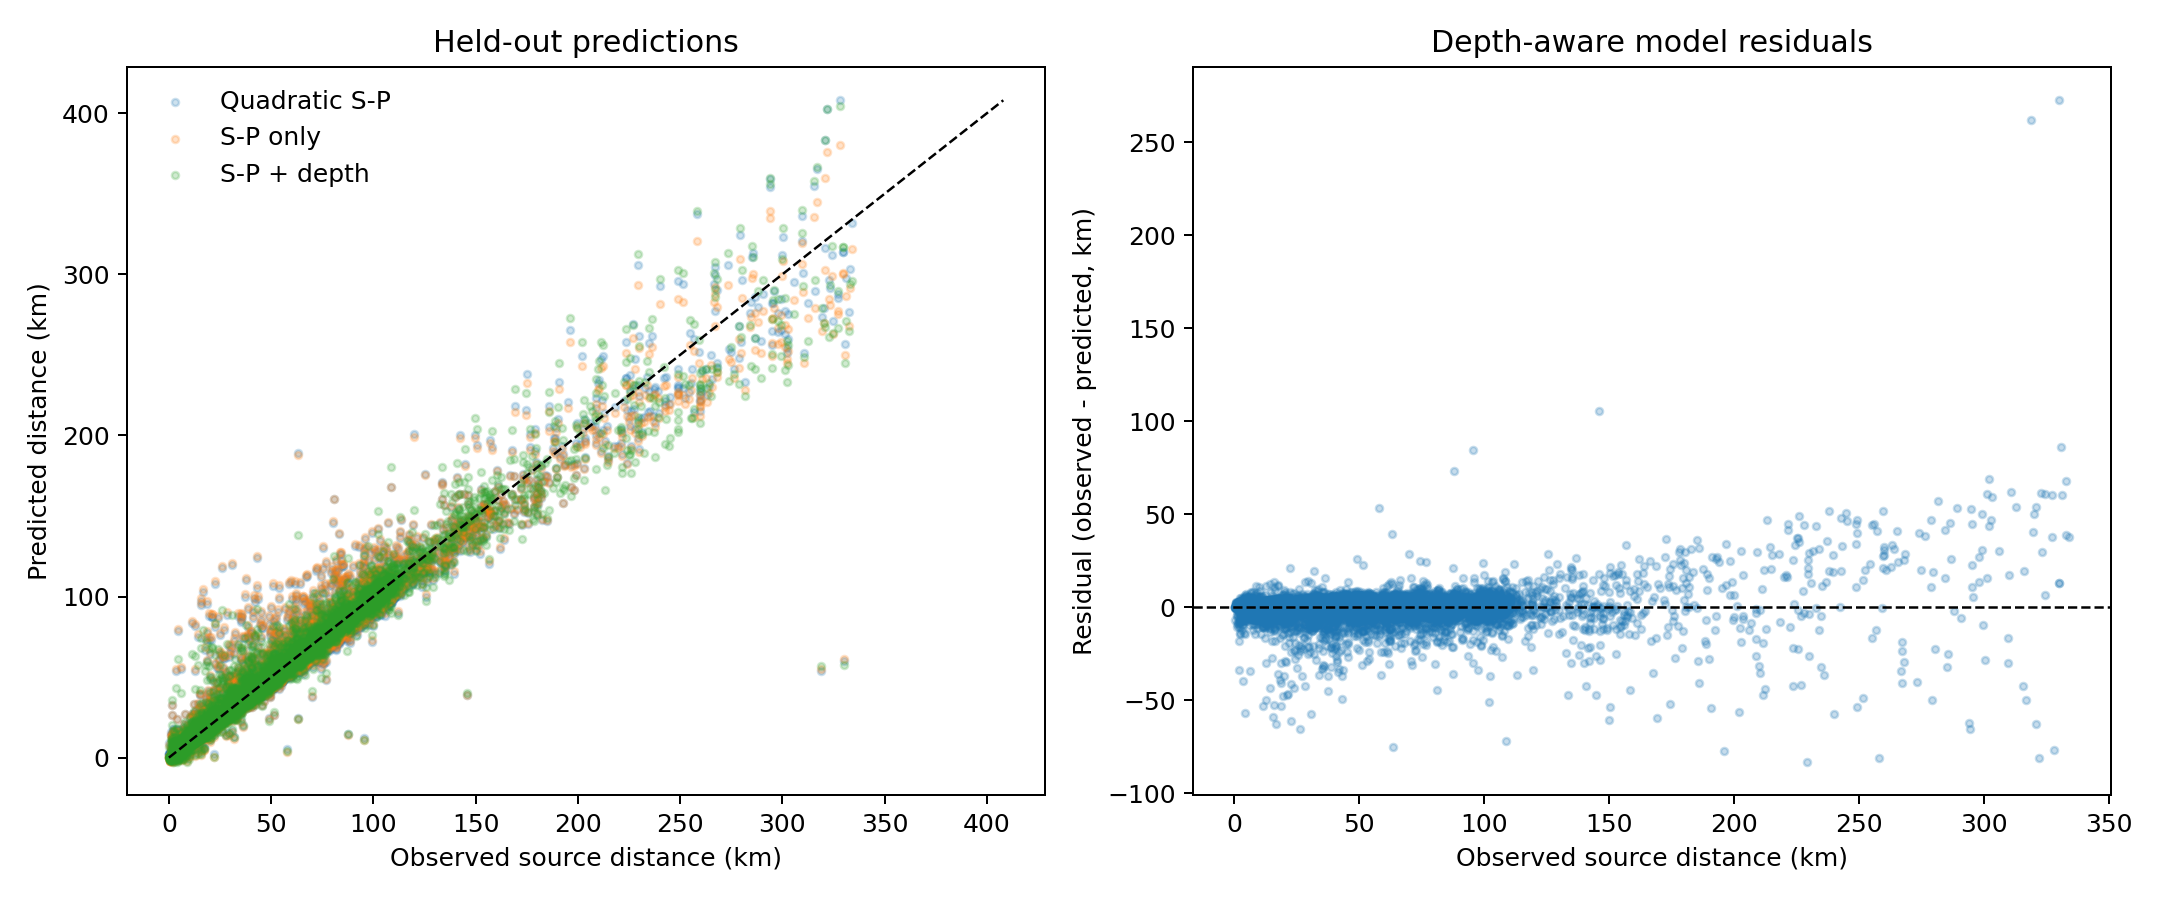
\includegraphics[width=\textwidth]{results/figures/rq1_distance_diagnostics.png}
  \caption{RQ1 held-out predictions from three fitted models (left) and residuals from the depth-aware model (right).}
  \label{fig:rq1}
\end{figure*}

For RQ2, the event-level model estimated a magnitude coefficient of 8.659 dB per ML unit (95\% CI: 8.613--8.705; $p<0.001$), after accounting for log-transformed distance and depth. The full model had an in-sample $R^2$ of 0.349 and RMSE of 8.70 dB across 259,817 events. Figure~\ref{fig:rq2} displays the event-level SNR values and the adjusted fitted relationship at median distance and depth.

\begin{table}[t]
  \centering
  \caption{RQ2 adjusted event-level regression summary.}
  \label{tab:rq2}
  \begin{tabular}{@{}lr@{}}
    \toprule
    Quantity & Estimate \\
    \midrule
    Magnitude coefficient (dB/ML) & 8.659 \\
    95\% confidence interval & [8.613, 8.705] \\
    Events & 259,817 \\
    In-sample $R^2$ & 0.349 \\
    In-sample RMSE (dB) & 8.697 \\
    Model-based $p$-value & $<0.001$ \\
    \bottomrule
  \end{tabular}
\end{table}

\begin{figure}[t]
  \centering
  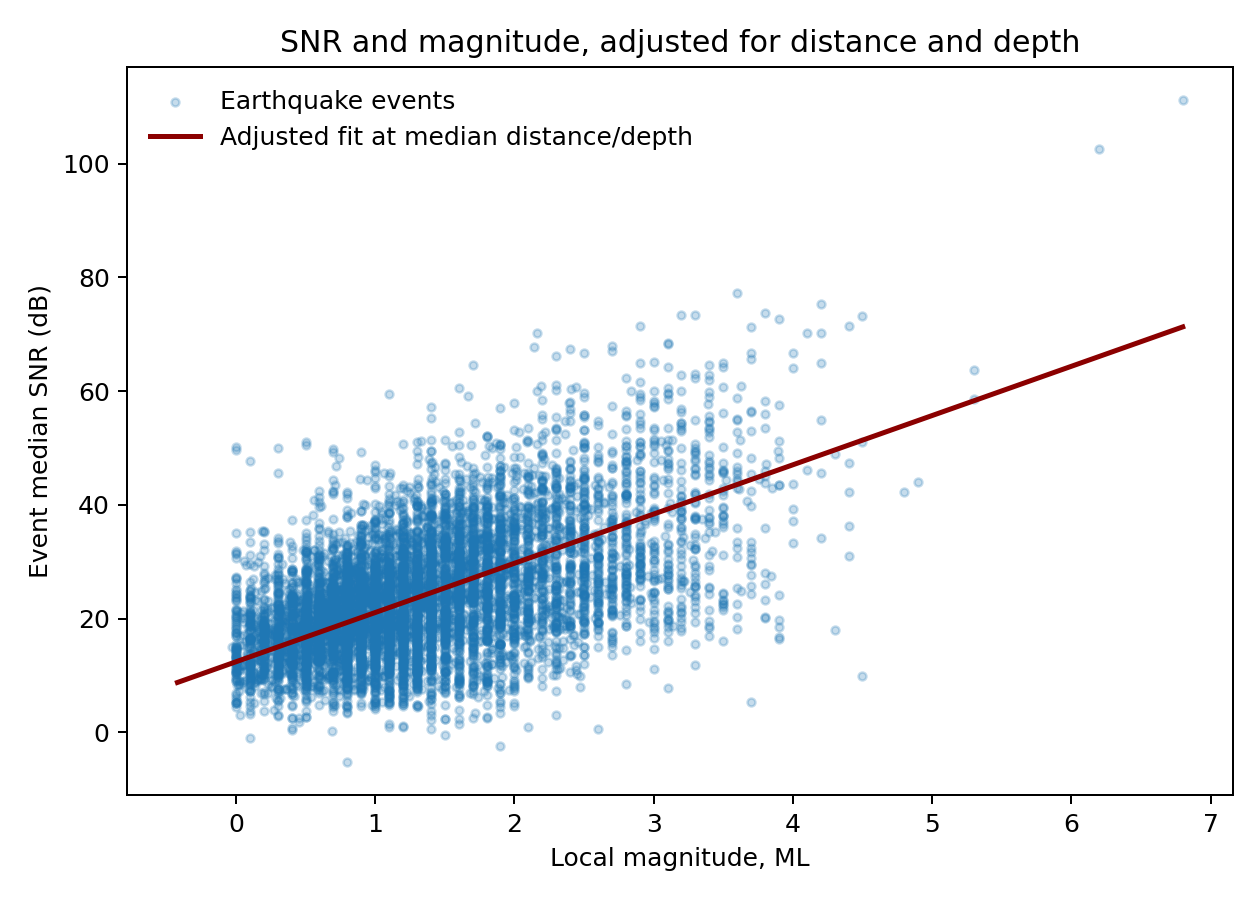
\includegraphics[width=\columnwidth]{results/figures/rq2_snr_magnitude.png}
  \caption{Event-level median SNR against local magnitude, with the fitted magnitude relationship evaluated at median distance and depth.}
  \label{fig:rq2}
\end{figure}

\section{Discussion}
The held-out results indicate that S--P time alone contains substantial information about source distance in this dataset. Adding depth improved all three reported metrics relative to the timing-only linear model. The quadratic timing-only fit produced only a small RMSE improvement and a slightly worse MAE, so curvature alone did not match the gain from including depth. The residual plot also shows increasing spread and notable outliers at larger distances, which limits the accuracy of this simple global calibration.

The positive adjusted magnitude coefficient is consistent with larger events tending to have higher SNR, while the negative distance coefficient is consistent with signal quality decreasing with propagation distance. The model's $R^2$ of 0.349 shows that magnitude, distance, and depth leave substantial SNR variation unexplained. Station and instrument properties, regional attenuation, local noise, phase-pick quality, and event clustering may contribute. Confidence intervals and $p$-values are model-based; aggregation removes repeated station traces within each event but does not account for dependence among related events or all heteroscedasticity.

This study analyzes metadata only. It cannot inspect waveform shape, recompute SNR, verify phase picks from traces, or apply FFT. The results also depend on STEAD's global mixture of networks, the chosen ML-only subset for RQ2, and the dataset's supplied event labels. A next step would be to repeat the analysis on a manageable HDF5 waveform subset, compare results across regions or station types, and assess phase-pick status and SNR definitions directly.

\section{Conclusion}
On a source-ID-separated test split, adding source depth improved P--S-based distance estimates over linear and quadratic timing-only fits. In an event-level ML subset, magnitude remained positively associated with median SNR after controlling for distance and depth, although the metadata-only model left substantial variation unexplained.

\section{Reproducibility}
The code, pinned analysis dependencies, metadata archive, tables, and figures are in the project directory. From the repository root, install dependencies with \texttt{pip install -r requirements.txt}, then reproduce all tables and figures with \texttt{XDG\_CACHE\_HOME=/tmp/snakemake-cache snakemake --cores 1}. On systems with a writable user cache, \texttt{snakemake --cores 1} is sufficient. The public GitHub repository link will be added here after publication: \texttt{[repository URL]}. The same dataset link is in the repository README.

\section{Contribution Statement}
\begin{table}[t]
  \centering
  \caption{Team contributions. Replace the placeholders with accurate contributions.}
  \label{tab:contributions}
  \begin{tabular}{@{}ll@{}}
    \toprule
    Team member & Contribution \\
    \midrule
    [Member 1] & [TODO] \\
    [Member 2] & [TODO] \\
    [Add rows as needed] & [TODO] \\
    \bottomrule
  \end{tabular}
\end{table}

\section{AI Usage Disclosure}
OpenAI Codex was used to brainstorm the research questions, inspect and analyze the supplied metadata, generate and run the Python analysis code, create the analysis tables and figures, draft this manuscript, and prepare project documentation. The team should review the code and calculations, independently reproduce the outputs, and revise the paper to reflect its own verified understanding. Any further AI assistance used by a team member must be added to this disclosure.

\begin{thebibliography}{9}

\bibitem{stead}
S. M. Mousavi, Y. Sheng, W. Zhu, and G. C. Beroza. 2019.
STanford EArthquake Dataset (STEAD): A Global Data Set of Seismic Signals for AI.
\textit{IEEE Access} 7, 179464--179476.
DOI: \url{https://doi.org/10.1109/ACCESS.2019.2947848}.

\bibitem{kaggle}
Kaggle user isevilla. \textit{Stanford Earthquake Dataset (STEAD)}. Kaggle.
\url{https://www.kaggle.com/datasets/isevilla/stanford-earthquake-dataset-stead?resource=download}.

\bibitem{holmgren}
J. M. Holmgren, M. J. Werner, K. Goda, M. Villani, V. Silva, P. Chindandali,
and V. Stevens. 2023. A relocated earthquake catalog and ground motion database
for the southern East African rift system. \textit{Earthquake Spectra} 39(3),
1911--1929. DOI: \url{https://doi.org/10.1177/87552930231173450}.

\bibitem{kwiatek}
G. Kwiatek and Y. Ben-Zion. 2016. Theoretical limits on detection and analysis
of small earthquakes. \textit{Journal of Geophysical Research: Solid Earth}
121, 5898--5916. DOI: \url{https://doi.org/10.1002/2016JB012908}.

\end{thebibliography}

\end{document}
